\section{Comparison with the original publication}
\label{sec:comparison}

This section compares the replication directly with what \citet{brignone2025} publish, side by side and with explicit deviations. It is distinct from the outturn comparison of Section~\ref{sec:results}: Table~\ref{tab:quarterly} there judges the model's forecasts against subsequent ONS data, whereas everything here judges the replication against the \emph{paper's own published numbers and figures}.

\subsection{Published anchors, side by side}
\label{sec:comparison-table}

The paper publishes two quantitative anchors that the replication's test suite locks against --- the one-year global FEVD shares of UK GDP and UK CPI --- plus a set of qualitative results (restriction patterns, the unrestricted oil-price sign check, the shock narrative, and the ranking of domestic CPI contributors). Table~\ref{tab:pubcompare} collects all of them. Two replication configurations are shown: the CI fast configuration (600 posterior draws, fixed seeds, 51 accepted, unweighted --- exactly the configuration the repository's validation tests run on every commit) and the production configuration (10{,}000 draws, 744 accepted, importance-weighted, ESS 356.1). Both are computed on the paper's own definition of the statistic, set out in Section~\ref{sec:validation}: the posterior mean of the group share formed on each accepted draw, at the four-quarter-ahead forecast-error variance, as a share of total variance.

\begin{table}[t]
\centering
\caption{Replication versus the published values of \citet{brignone2025}}
\label{tab:pubcompare}
\footnotesize
\begin{tabularx}{\textwidth}{@{}>{\raggedright\arraybackslash}Xllll@{}}
\toprule
Quantity & Paper & Fast config & Production & Deviation \\
\midrule
Global share, UK GDP FEVD, 1 yr & $\sim$40\% & 42.0\% & 37.4\% & $+2.0$ / $-2.6$ pp \\
Global share, UK CPI FEVD, 1 yr & $\sim$50\% & 37.6\% & 42.3\% & $-12.4$ / $-7.7$ pp \\
Identified total, UK GDP / CPI, 1 yr & ``around 80\%'' & --- & 76\% / 79\% & $-4$ / $-1$ pp \\
Oil-price impact IRF, world supply shock & positive (Fig.~2) & $+5.83$ & positive & sign matches \\
Zero restrictions (paper Table~2) & imposed & \multicolumn{2}{l}{hold exactly ($<10^{-9}$), every draw} & cannot fail \\
Sign restrictions (paper Table~2) & imposed & \multicolumn{2}{l}{hold on every accepted draw} & cannot fail \\
Sign restrictions, median IRF & imposed per draw & \multicolumn{2}{l}{hold} & none \\
Shock narrative episodes (paper Fig.~5) & 2008, 2022--23 & \multicolumn{2}{l}{reproduced} & none \\
CPI inflation surge attribution (paper Fig.~6) & global energy/demand & \multicolumn{2}{l}{reproduced} & none \\
Largest domestic CPI contributor & monetary policy (prose) & \multicolumn{2}{l}{UK supply (13.9\% vs 8.7\%)} & unresolved \\
UK GDP IRF to world shocks, long horizons & persistently positive & \multicolumn{2}{l}{median decays through zero} & inside bands \\
\bottomrule
\end{tabularx}
\par\smallskip
\parbox{0.97\textwidth}{\footnotesize \emph{Notes:} ``Fast config'': 600 posterior draws, sample seed 1, identification seed 2, 51 accepted, unweighted --- the repository's per-commit CI validation configuration, re-estimated fresh for this table by \texttt{figures/make\_comparison.py}. ``Production'': 10{,}000 draws, 744 accepted, importance-weighted (ESS 356.1), from the repository's production artifact. FEVD rows are posterior means of the per-draw group share of \emph{total} four-quarter-ahead forecast-error variance, the statistic the paper's Figure~4 plots; the production 68 per cent posterior bands are $[23.4, 52.2]$ for GDP and $[25.5, 60.3]$ for CPI, so the deviations shown are well inside a single band. Deviations are fast~/~production in percentage points against the paper's approximate published shares. The zero and sign restriction rows are marked ``cannot fail'': they are properties of the \citet{arias2018} construction and of the accept/reject rule, not tests. The paper publishes IRFs only as figures --- no numeric values --- so IRF comparisons are of sign and shape. The domestic-contributor row is marked unresolved: the paper asserts the ranking in prose but publishes no FEVD table.}
\end{table}

The headline pattern is a partial match, and less flattering than earlier versions of this table reported. On UK GDP the production run's 37.4 per cent against the paper's $\sim$40 is a match, and the total explained by the six identified shocks (76 and 79 per cent against ``around 80'') lines up on both variables. On UK CPI the replication finds 42.3 per cent against $\sim$50 --- roughly eight points short. Earlier versions of this paper reported 42.1 and 49.5 per cent and read the CPI figure as a match to within half a point; that agreement was produced by renormalising a sum of per-shock posterior medians to 100 per cent, an arithmetic step rather than an economic result (Section~\ref{sec:validation}).

Two things stop the shortfall being over-read. First, the 68 per cent posterior band on the CPI share is $[25.5, 60.3]$, about $\pm14$ points --- wider than the eight-point gap, so the data do not resolve it. Second, the difference between the fast and production configurations (42.0 versus 37.4 for GDP, 37.6 versus 42.3 for CPI) is Monte-Carlo noise in a 51-draw accepted sample, not a weighting effect: the global GDP share from the fast configuration has a standard deviation of about 6.5 points across sampling seeds, and the unweighted 3{,}000-draw run behind Figures~\ref{fig:irf}--\ref{fig:hd} lands at 38.1 and 42.3 per cent, within a point of the weighted production values. An earlier version of this section claimed the importance weights moved both shares substantially towards the published values; on the corrected statistic they do not, and the weights' role is the narrower one of correcting the \citet{arias2018} zero-restriction sampler towards the uniform-over-rotations posterior.

Figure~\ref{fig:comparison} shows the same comparison graphically. No ours-versus-paper IRF overlay is drawn because \citet{brignone2025} publish impulse responses only as figures; neither the paper nor the repository's validation data contains digitised numeric IRF paths, so the IRF comparison is confined to the sign and shape checks in Table~\ref{tab:pubcompare} and Section~\ref{sec:validation}.

\begin{figure}[t]
\centering
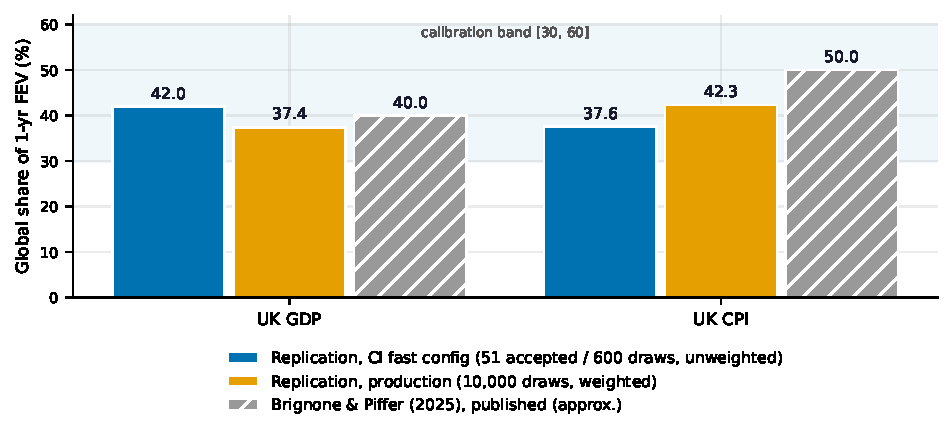
\includegraphics[width=0.82\textwidth]{figures/fig_comparison.pdf}
\caption{One-year global FEVD shares of UK GDP and UK CPI: replication versus \citet{brignone2025}. Shares are posterior means of the per-draw group share of total four-quarter-ahead forecast-error variance --- the statistic the paper's Figure~4 plots --- and are not renormalised. Blue: fresh fixed-seed run of the CI fast configuration (600 draws, 51 accepted, unweighted). Orange: production run (10{,}000 draws, 744 accepted, importance-weighted). Hatched grey: the paper's approximate published values. Shaded region: the $[30,60]$ per cent regression tripwire used by the validation suite, which is too wide to constitute a calibration result.}
\label{fig:comparison}
\end{figure}

\subsection{The companion Staff Working Paper on structural forecast analysis}
\label{sec:comparison-swp}

The natural question after Table~\ref{tab:quarterly} is whether the model's authors have published forecast-evaluation numbers of their own to compare against. The companion paper --- \citet{brignone2026}, Bank of England Staff Working Paper No.~1{,}165, ``Structural forecast analysis'', January 2026 --- turns out to answer a different question. It is a methods paper: it derives a five-way structural decomposition of forecast errors and forecast revisions (deterministic component, past shocks, revisions to past shocks, new shocks, and parameter/vintage revision) and illustrates it on a \emph{four}-variable UK SVAR (Bank Rate, real GDP, CPI and real oil prices, 1992Q1--2025Q2, five lags, hierarchical \citealp{giannone2015} hyperpriors, Covid dummies for 2020), running real-time unconditional forecasts each quarter from 2021Q4 to 2025Q2 on the actual ONS vintages. It publishes no root-mean-squared errors, coverage rates or benchmark comparisons --- its output is the structural attribution of the errors, shown in figures --- so no numeric accuracy comparison with Table~\ref{tab:quarterly} is possible, and the RMSEs reported there (0.32 percentage points at horizons of one to seven quarters) stand without an official counterpart.

The comparison that \emph{is} possible is of the attribution itself, and it is reassuring. \citet{brignone2026} attribute the large upward inflation-forecast revisions of 2022 to inflationary supply and energy shocks combined with expansionary demand and monetary policy shocks, plus revisions to previously estimated shocks. The replication's forecast-revision machinery (Section~\ref{sec:forecasting-math}) is exactly the ``new shocks'' term of their five-way decomposition --- the term their identity isolates when the parameters and past data are held fixed --- and its 2024Q2 reading (a probable contractionary world energy shock alongside strong world demand, Section~\ref{sec:results}) is the same shock vocabulary applied two years later. Their broader decomposition, which also tracks vintage revisions and re-estimation, is a natural extension of the replication's fixed-parameter identity~\eqref{eq:revision}.

\subsection{Cross-checks against other published UK shock estimates}
\label{sec:comparison-shocks}

A replication of a set-identified SVAR should also be checked \emph{sideways}, against shock estimates published by other authors with different identification schemes. Table~\ref{tab:shockcompare} performs the check qualitatively --- sign and timing over the major overlapping episodes --- against three benchmarks: the Bank's own Monetary Policy Report narrative (most recently the November 2025 Report's quantified account of the 2025 inflation overshoot), the oil-supply-news series of \citet{kanzig2021}, identified from futures-price movements in tight windows around OPEC announcements (extended vintage through 2022), and the narrative UK monetary policy shock series of \citet{cloyne2016}.

\begin{table}[t]
\centering
\caption{Sign and timing of identified shocks across published UK estimates}
\label{tab:shockcompare}
\footnotesize
\begin{tabularx}{\textwidth}{@{}l>{\raggedright\arraybackslash}X>{\raggedright\arraybackslash}X>{\raggedright\arraybackslash}X@{}}
\toprule
Episode & This replication & Bank MPR narrative & \citet{kanzig2021} oil-supply news \\
\midrule
2008--09 crisis & Large negative world demand shocks & Global demand collapse & No large supply-news events; oil swings demand-driven --- consistent \\
\addlinespace
Covid, 2020 & Shocks muted by construction (Covid dummies absorb 2020Q1--2021Q2) & Unprecedented demand and supply disruption & 2020 oil crash read as demand, not supply news; April 2020 OPEC+ cut a positive supply-news event \\
\addlinespace
2021--23 energy crisis & Contractionary world energy shocks dominate the CPI decomposition (Figure~\ref{fig:hd}) & ``Imported inflation'': energy and tradables & Only modest shocks: the Russian gas shock fell outside OPEC announcement windows --- complementary, not contradictory \\
\addlinespace
2025 inflation hump & Energy/supply-side price shocks on weak demand (2024Q2 posterior reading, extended) & Nov 2025 MPR: 1.8 pp overshoot $=$ 0.4 pp administered prices $+$ 0.4 pp food $+$ $\sim$1 pp labour costs & Outside the series' 2022 data edge \\
\bottomrule
\end{tabularx}
\par\smallskip
\parbox{0.97\textwidth}{\footnotesize \emph{Notes:} Qualitative comparison of sign and timing; the underlying series use different identification schemes (zero/sign restrictions here; narrative decomposition in the MPRs; high-frequency futures surprises around OPEC announcements in \citealp{kanzig2021}). The \citet{cloyne2016} narrative UK monetary policy series is omitted from the episode columns because it ends in the 2000s (extended to early 2009, when Bank Rate reached its effective lower bound) and so overlaps none of the episodes; it and the high-frequency UK series of \citet{cesabianchi2020} (through 2015) remain the natural benchmarks for the replication's monetary policy shock over the pre-Covid sample.}
\end{table}

Three points deserve emphasis. First, where the schemes measure the same object --- the 2008 world demand collapse, the 2022 energy shock --- signs and timing agree. Second, where they measure \emph{different} objects the disagreement is informative rather than troubling: the replication's world energy shock is defined by price--quantity comovement across all energy-price drivers, so it registers the 2022 Russian gas shock strongly, while the OPEC-announcement instrument of \citet{kanzig2021} is deliberately silent on non-OPEC events. Third, the November 2025 MPR's arithmetic of the 2025 overshoot --- roughly half administered prices and food, half labour costs --- maps into the model's vocabulary as domestic cost-push (negative UK supply) layered on imported price shocks, which is precisely the shock combination the frozen 2024Q2 data edge could not yet see; it explains \emph{which} shocks the undershoot in Table~\ref{tab:quarterly} missed, not just that some were missed.

\subsection{The Bank's use of the model since publication}
\label{sec:comparison-use}

Two 2026 Bank publications confirm that the replicated model remains in operational use. The January 2026 \emph{Forecast Evaluation Report} lists \citet{brignone2025} among the ``range of cross-check models \ldots{} used regularly to help inform judgements and in some cases also interpret changes in the Bank's forecasts'' \citep{boe2026fer}. And in July 2026, MPC member Catherine L.\ Mann cited the companion methodology directly: ``Using a structural VAR model, Brignone and Piffer (2026) demonstrate that upward revisions in inflation forecasts following the post-pandemic inflation surge can be attributed to a combination of expansionary shocks on the demand side, revisions to past shocks, and contractionary supply-side shocks'' \citep{mann2026} --- the same attribution the replication's historical decomposition delivers for 2021--23 (Figure~\ref{fig:hd}).

The Bank's own published projections also provide a late cross-check on Table~\ref{tab:quarterly}. The February 2026 Monetary Policy Report put four-quarter CPI inflation at 3.0 per cent and four-quarter GDP growth at 0.8 per cent for 2026Q1 \citep{boe2026mpr_feb} --- forecasts made with seven more quarters of data than the replication's frozen 2024Q2 edge. The outturns were 3.1 and 0.9; the replication's eighteen-month-old medians were 3.2 and 0.9. For that quarter, at least, freezing the data edge in mid-2024 cost the model almost nothing relative to the official forecast made contemporaneously.
